\documentclass[crop,tikz,convert=pdf2svg,border=3mm]{standalone}

% Tikz settings optimized for causal graphs.
\usetikzlibrary{shapes,decorations,arrows,calc,arrows.meta,fit,positioning}
\tikzset{
	-Latex,auto,node distance =1 cm and 1 cm,semithick ,
	state/.style ={ellipse, draw, minimum width = 0.7 cm},
	point/.style = {circle, draw, inner sep=0.04cm,fill,node contents={}},
	bidirected/.style={Latex-Latex,dashed},
	el/.style = {inner sep=2pt, align=left, sloped}
}

\begin{document}
	
	% The graph
	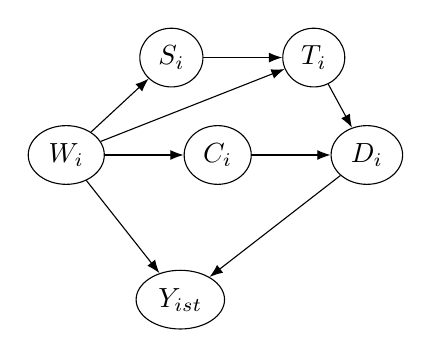
\begin{tikzpicture}
	\node[state] (1) {$W_i$};
	\node[state] (2) [right =of 1] {$C_i$};
	\node[state] (3) [right =of 2] {$D_i$};
	\node[state] (4) [above right =of 1,xshift=-0.3cm,yshift=-0.3cm] {$S_i$};
	\node[state] (5) [right =of 4] {$T_i$};
	\node[state] (6) [below right =of 1,xshift=-0.3cm,yshift=-0.3cm] {$Y_{ist}$};
	
	\path (1) edge node[above] {} (2);
	\path (1) edge node[above] {} (5);
	\path (1) edge node[above] {} (6);
	\path (2) edge node[above] {} (3);
%	\path[bidirected] (2) edge[bend left=60] node[above] {$\epsilon_{xy}$} (3);
	\path (1) edge node[el,above] {} (4);
	\path (4) edge node[el,above] {} (5);
	\path (5) edge node[el,above] {} (3);
	\path (3) edge node[el,above] {} (6);
%	\path[bidirected] (4) edge[bend left=50] node[el,above] {$\epsilon_{wy}$} (3);
	\end{tikzpicture}
	
\end{document}